\documentclass[12pt,letterpaper,twoside]{amsart}
\usepackage[latin1]{inputenc}
\usepackage{amsmath}
\usepackage{amsfonts}
\usepackage{graphicx}
\usepackage{amssymb}
\usepackage{multicol}
\usepackage{ulem}
\newcounter{example}
\newcounter{exercise}
\newcounter{problem}
\newtheorem{theorem}{Theorem}
\newcommand{\example}{\bigskip \noindent {\large {\sc Example \arabic{example}:}} \addtocounter{example}{1}}
\newcommand{\exercise}{\bigskip \noindent {\large {\sc Exercise \arabic{exercise}:}} \addtocounter{exercise}{1}}
\newcommand{\problem}{\bigskip \noindent {\large {\sc Problem \arabic{problem}:}} \addtocounter{problem}{1}}
\newcommand{\tech}{\marginpar{\vskip 10mm \begin{center}\includegraphics[width=0.25in]{calculatorimagesmall.eps} \end{center}}}
\newcommand{\solution}{\medskip \noindent {\bf Solution: }}
\newcommand{\R}{\mathbb{R}}





\begin{document}

\sffamily

%%%%  switch the commenting on this line and the next \chapter{Introduction}
\begin{center} {\LARGE Numerical Methods} \end{center}

\setcounter{example}{1}
\setcounter{exercise}{1}

In this chapter, we wil discuss a method for finding approximate values of solutions to ODE even when it is not possible to find formulas for solutions analytically.

The first example below will illustrate the basic idea of our approach, and the second example will demonstrate the fully developed idea.

\example Consider the initial value problem
\[ \left\{ \begin{matrix} y'=y^2-x \\ y(0)=1 \end{matrix} \right.\]
Suppose we want to know the value of $y(1)$, but we are unable to calculate an exact solution for the ODE.  We can still find an approximate solution as follows.

If $y(x)$ is the solution, then the initial condition implies that $y(0)=1$, and if we insert $x=0$ and $y=1$ into the differential equation, that tells us that $y'(0)=(y(0))^2-(0)=(1)^2-0=1$.  Therefore the tangent line approximation to $y(x)$ at the point $(0,1)$ is 
\[ y(x) \approx x+1.\]
Therefore we can deduce that $y(1)\approx 2$.
\qed

This picture illustrates the solution curve and the tangent line in the first example:
\begin{center}
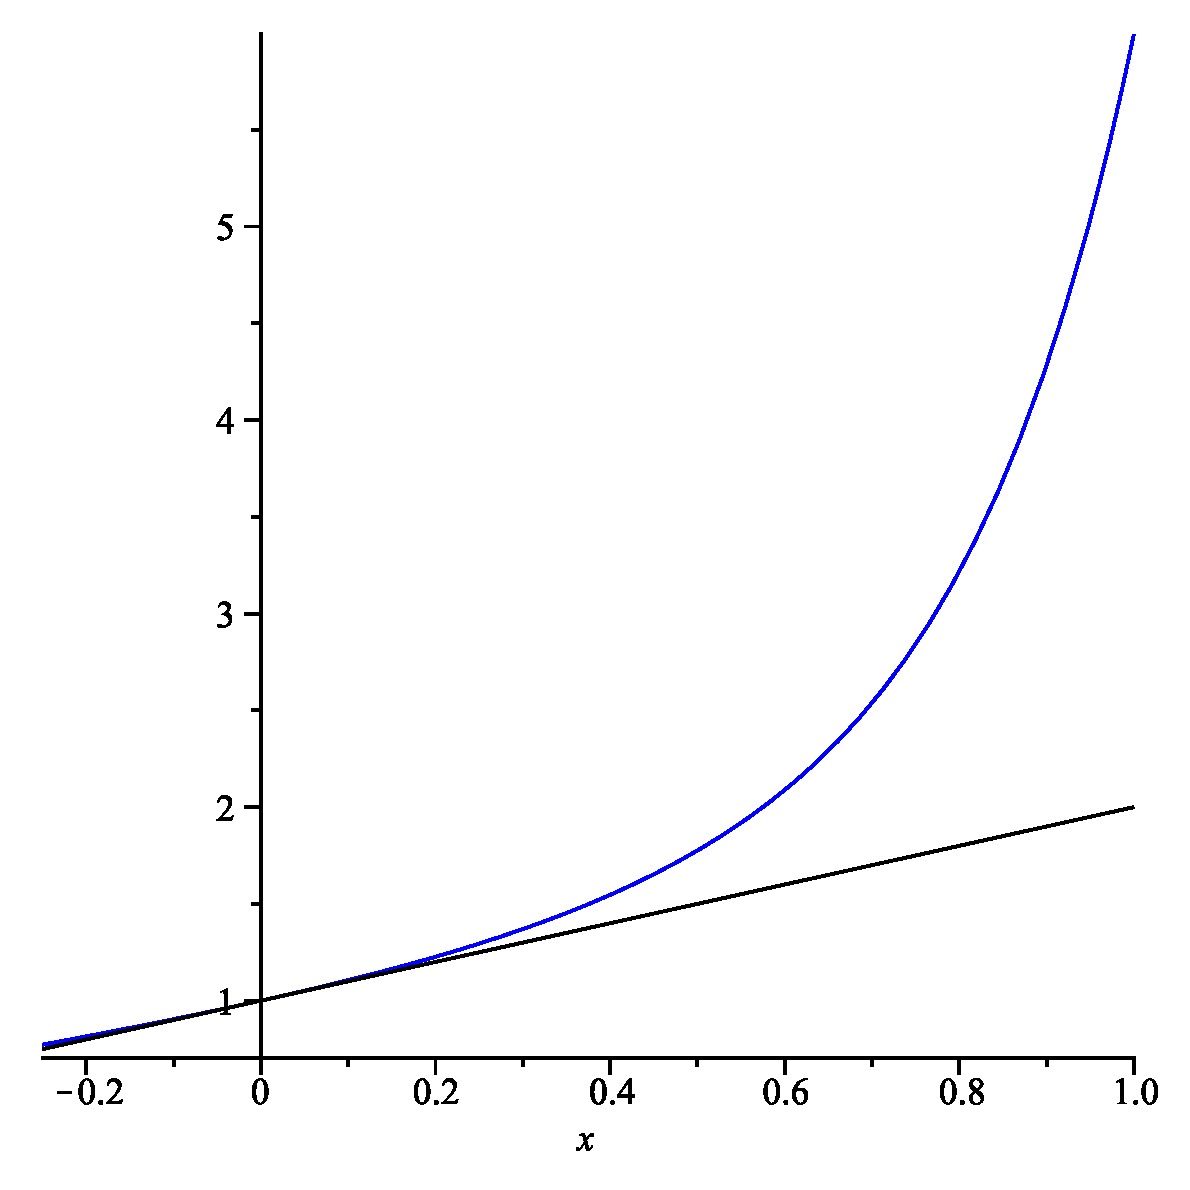
\includegraphics[width=3in]{example1.eps}
\end{center}
The idea was that, because we know the slope of the solution curve at the initial point $(0,1)$, we can use that to project what happens as $x$ increases.  However, it is not hard to see that the linear approximation is only good for small values of $x$ -- the actual solution curve grows quickly as $x$ increases, and the difference between the curve and the tangent line will only worsen away from the initial point.

One way to compensate for this is to use a different type of approximation -- a piecewise linear one.

Instead of following the tangent line all the way to the point where $x=1$, let's just follow it until $x=0.5$; then, at that point, we'll recompute the slope based on the differential equation.  According to the tangent line approximation, when $x=0.5$, we get $y \approx 1.5$; inserting this into the differential equation gives us $y' \approx (1.5)^2-(0.5)=1.75.$  This becomes the slope for the segment from $x=0.5$ to $x=1$:
\begin{center}
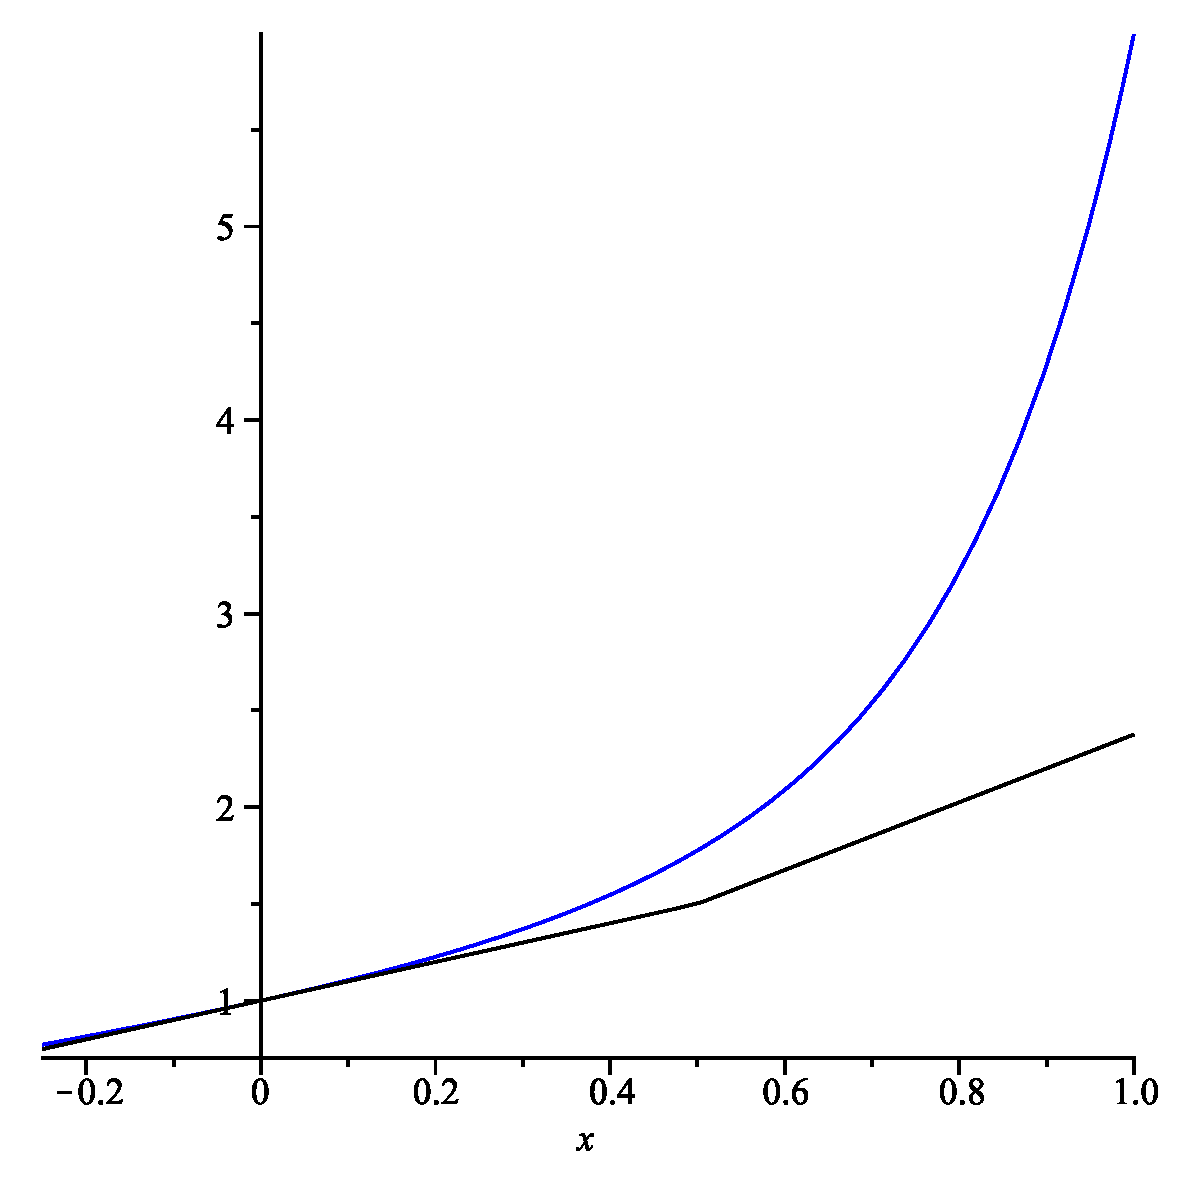
\includegraphics[width=3in]{example2.eps}
\end{center}
Based on this, we estimate that $y(1) \approx 1.5+0.5((1.5)^2-0.5))=2.375$.  Now our approach for finding an approximate solution has taken shape: by using a finer subdivision of intervals, we can obtain a better approximation for the value of $y(1)$.  The following graph shows how dividing the interval $[0,1]$ into 4 subintervals gives an even better approximation:





%% Cut below here for the book form.

\begin{center} {\LARGE Problems} \end{center}

\setcounter{problem}{1}

\problem Consider the following initial value problem: $y'=y, \ y(0)=y_0$.  {\bf (a)} Use Euler's method to find an approximate value for $y(x)$ by dividing the interval $[0,x]$ into $N$ subintervals of equal width.  (That is to say, you will use $\Delta x = \frac{x}{N}$.  {\it (Hint: Verify that $y_i=y_0(1+\Delta x)^i$.)}  {\bf (b)} Take a limit of the result in (a) as $N \rightarrow \infty$ to get the exact value of $y(x)$.






\end{document}